\section{Formal Definitions and Proofs}
\label{sec:proofs}

\subsection{Graph definitions}

We begin this section by formally defining the graphs and graph instances used in our algorithm as fundamental structures.
\begin{definition}{Typed Graph}
\label{def:typed_graph}
A typed graph is a triple $\langle V,E,\tau\rangle$ where $V$ is a finite set of
vertices, $E\subseteq V\times V$ is a set of edges connecting the vertices and
$\tau:V\rightarrow Type$ is a typing function for the elements of V, where $Type$ is
a set of type names. Edges $(v,v')\in E$ are noted $v\rightarrow v'$. The set of
all typed graphs is called $TG$.
\end{definition}

Definition~\ref{def:typed_graph_homomorphism} describes when a typed graph is said to be homomorphic to another.

\begin{definition}{Typed Graph Homomorphism  / Typed Graph Instance}
\label{def:typed_graph_homomorphism}

Let $\langle V,E,\tau\rangle=g,\langle V',E',\tau'\rangle=g'\in TG$ be typed
graphs. There is a typed graph homomorphism between $g'$ and $g$ if and only if
there exists a graph homomorphism $f:V'\rightarrow V$ such that for all $v'\in
V$ we have that $\tau'(v')=\tau(f(v'))$. Note that, trivially, a typed graph
homomorphism is a formal homomorphism. We denote an \emph{injective} typed graph
homomorphism between typed graphs $g$ and $g'$ by $g' \vartriangleleft g$.
\end{definition}

In the text that follows we will use the terms \emph{typed graph homomorphism}
and \emph{typed graph instance} interchangeably.

Definition~\ref{def:typed_graph_strict_instance} is stricter than
definition~\ref{def:typed_graph_homomorphism}, and indicates that there is a
strict many-to-one type correspondence of the nodes of two graphs and their
relations.

\begin{definition}{Typed Graph Strict Instance}
\label{def:typed_graph_strict_instance}

Let $\langle V,E,\tau\rangle=g,\langle V',E',\tau\rangle=g'\in TG$ be typed
graphs. $g'$ is a typed graph strict instance of $g$, noted $g'
\blacktriangleleft g$, if and only if there exists a surjective
typed graph homomorphism between $g'$ and $g$.

\end{definition}

In order to simplify the subsequent development we will often
use the notation ${\langle V,E,\tau\rangle}^*$ to represent the transitive
closure of the edges of typed graph  $\langle V,E,\tau\rangle$.

\subsection{Required Component Definitions}

Following along from our definition of the graphs used in our algorithm, this section then builds these graphs into the required structures.

\begin{definition}{Metamodel}
\label{def:metamodel}

A metamodel $\langle V,E,\tau\rangle\in TG$ is a typed graph where $\tau$ is a bijective typing function. The set of all metamodels is called META.

\end{definition}

Definition~\ref{def:metamodel} formally states that a metamodel corresponds to a graph of typed elements where only one element for each type is represented. This definition is then used to state definition~\ref{def:pattern}, where a typed graph is combined with its metamodel.

\begin{definition}{Pattern\footnote{Note that we the definition of pattern corresponds to the formal definition of \emph{Model} (definition 5) in our previous work presented in~\cite{Lucio:10}. The renaming was done in an effort to construct a more appropriate vocabulary to better describe our technique.}}
\label{def:pattern}

A pattern is a 4-tuple $\langle V,E,\tau,M\rangle$, where $\langle
V,E,\tau\rangle$ is a typed graph. Moreover $M=\langle V',E',\tau'\rangle\in
META$ is a metamodel and the codomain of $\tau$ equals the codomain of $\tau'$.
We also have that $\langle V,E,\tau\rangle$ is a typed graph instance of a
metamodel $M$. The set of all patterns for a metamodel $M$ is called $PAT^{M}$.
\end{definition}

% \begin{figure}[h!] \centering \includegraphics[scale=.5]{./figures/model_instance_example.pdf}
% 	\caption{An Example of a Model, instance of a Metamodel}
% 	\label{fig:model_instance_example}
% \end{figure}

Match and apply graphs are constructs of DSLTrans and are informally described in section~\ref{subsec:DSLTrans_constructs} for DSLTrans rules and in section~\ref{subsubsec:path_condition_creation} for path conditions. These graphs are formalised in definition~\ref{def:match_apply_model}.

\begin{definition}{Match-Apply Pattern}
\label{def:match_apply_model} 

A match-apply pattern is a 5-tuple $\langle V,E,\tau, Match,Apply\rangle$,
where $Match=\langle V',E',\tau',s\rangle$ and $Apply=\langle
V'',E'',\tau'',t\rangle$ are patterns, $V=V'\cup V''$, $E= E'\cup E''$ and
$\tau=\tau'\cup \tau''$. $s$ is called the \emph{source} metamodel and $t$ the
target metamodel. The set of all match-apply patterns for a source metamodel $s$
and a target metamodel $t$ is called $MAP^{s}_{t}$.
%Vertices in the $Apply$ model which are not connected to \emph{backward links} are called \emph{free vertices}.
%We additionally define the $back:MAM^{s}_{t}\rightarrow MAM^{s}_{t}$ function
%which extends a match-apply model by adding edges that connect all vertices in
%the $Match$ model to all \emph{free} vertices.

\end{definition}
%(##) as several models are applied
%	match model created

Definition~\ref{def:path_condition} then defines a path condition to be largely constructed from a match graph, an apply graph, and traceability links between the graphs.

\begin{definition}{Path Condition}
\label{def:path_condition}

A Path Condition is a 7-tuple $\langle V,E\cup Tl\cup
Il,\tau,Match,Apply,Tl,Il\rangle$, where\\$\langle V,E,\tau,Match,Apply\rangle
\in MAP^{s}_{t}$ is a match-apply pattern. $Match=\langle V',E', \tau',s\rangle$,
$Apply=\langle V'',E'', \tau'',t\rangle$, the edges $Tl\subseteq V'\times V''$
are called \emph{traceability links} and the edges $Il\subseteq V'\times V'$ are
called \emph{indirect links}. The set of all path conditions having source
metamodel $s$ and target metamodel $t$ is called $PC^{s}_{t}$.
%We additionally define the $strip:TR^{s}_{t}\rightarrow TR^{s}_{t}$
%function which removes from a transformation rule all free vertices and
%associated edges.

\end{definition}

% The language to describe properties is in fact very similar to the language to
% express transformations, with the additional possibility of expressing indirect
% links in the $apply$ pattern --- thus allowing more abstract patterns than the
% ones expressed in transformations. This is natural given that the properties of
% a transformation can be more abstract than the rules implementing them.

A transformation execution is formed from taking the input model, and executing
the transformation on it to produce the output model. During this
transformation, traceability links will be placed between match elements and the
apply elements they create. Definition~\ref{def:transf_ex} expresses this
formally. Note that we assume that transformation executions are built following
the algorithm described in~\cite{DBLP:conf/sle/BarrocaLAFS10}.

\begin{definition}{Transformation Execution}
\label{def:transf_ex}

Let $t$ be a DSLTrans transformation having source metamodel $s$ and target
metamodel $t$. A Transformation Execution is a 6-tuple $\langle V,E\cup
Tl,\tau,Match,Apply,Tl\rangle$, where $\langle V,E,\tau,Match,Apply\rangle \in
MAP^{s}_{t}$ is a match-apply pattern. $Match=\langle V',E', \tau',s\rangle$,
$Apply=\langle V'',E'', \tau'',t\rangle$ and the edges $Tl\subseteq V'\times
V''$ are called \emph{traceability links}. The set of all transformation
executions having source metamodel $s$ and target metamodel $t$ is called
$Exec^{s}_{t}$.
\end{definition}

Definition~\ref{def:instance_pc_ex} is crucial to our work as it says that a path condition formally represents some number of concrete transformation executions. This will be used in the next section as a building block to say that properties proved on the path condition are also proved on the transformation executions it represents.  

\begin{definition}{Abstraction of a Transformation Execution by a Path Condition}
\label{def:instance_pc_ex}

Let $t$ be a DSLTrans transformation having source metamodel $s$ and target
metamodel $t$. Let also $pc = \langle
V_{pc},E_{pc},\tau_{pc},Match_{pc},Apply_{pc},Tl_{pc},Il_{pc}\rangle \in
PC^{s}_{t}$ of be a path condition and $ex = \langle
V_x,E_x,\tau_x,Match_x,Apply_x,Tl_x\rangle \in Exec^{s}_{t}$ be an execution of
$t$. Let also $Match_x = \langle V_{mx},E_{mx},\tau_{mx}\rangle$ and $Match_{pc}
= \langle V_{mpc},E_{mpc},\tau_{mpc}\rangle$. We have that $ex$ satisfies $pc$,
noted $ex\Vvdash pc$, if and only if:
$$Match_{pc} \vartriangleleft Match^*_x \;\land\; \langle V_x,E_x\setminus
E_{mx},\tau_x\rangle \blacktriangleleft \langle V_{pc},E_{pc}\setminus
E_{mpc},\tau_{pc}\rangle$$ More informally, there exists a typed graph injective
homomorphism between $Match_{pc}$ and $Match_x$ \levi{It is possible that this
relation is required to be a typed graph strict instance between the path
condition and the execution. Such a constraint would oblige each set of
executions for a path condition to be truly distinct from the set of executions
for another path condition. With the current definition the executions for a
path condition including rule 'A' will overlap with the executions for a path
condition including rules 'AB'. If this is so validity needs to be proved again
for the new relation between the match patterns of PC and ex. Elements that do
not show up in the match part of the rules are excluded from the typed graph
strict instance.}  \textbf{and} $\langle V_x,E_x\setminus E_{mx},\tau_x\rangle$
is a typed graph strict instance of $\langle V_{pc},E_{pc}\setminus
E_{pc},\tau_{pc}\rangle$.

\end{definition}

Note that in definition~\ref{def:instance_pc_ex} the match associations are naturally excluded from the typed strict instance relation between the apply pattern of the transformation execution and the apply pattern of the path condition. Vertices of match patterns are nonetheless kept. This is so because traceability links need to be considered in the typed graph strict instance relation as well as, together with those traceability links, the vertices of the match patterns.  

%\levi{Is this where we want to mention one execution is covered by one/more than one path condition?}

% In figure~\levi{add a figure depicting the surjective graph homomorphism here}
% we depict the relation between a path condition and a transformation execution.

\subsection{Validity and Completeness of the Property Proving algorithm}

This section will use the above definitions in order to prove the validity and completeness of our property proof algorithm presented in section~\ref{sec:verif_dsltrans_props}. %Note that we make the following assumptions:

% \levi{Fix}
% \begin{itemize}
%   \item Edge types are disregarded
%   \item Transformation executions are correctly built given a transformation (as per SLE paper)
%   \item Path conditions are correctly built given a transformation (as described in this paper)
%   \item Mention notational differences with previous papers and why they were introduced
%   \item We do not present the formal definition of transformation here and refer the reader to the SLE paper
% \end{itemize}


The structure of a transformation property is formally defined in definition~\ref{def:trans_prop}. As with most other constructs in our algorithm, it is also formed from a match graph and an apply graph.

\begin{definition}{Property of a Transformation}
\label{def:trans_prop}

Let $t$ be a DSLTrans transformation having source metamodel $s$ and target
metamodel $t$. A property of $t$ is a 7-tuple $\langle V,E\cup
Il,\tau,Match,Apply,Bl,Il\rangle$, where \\$\langle V,E,\tau,Match,Apply\rangle
\in MAP^{s}_{t}$ is a match-apply pattern. $Match=\langle V',E',\tau',s\rangle$,
$Apply=\langle V'',E'',\tau'',t\rangle$, the edges $Tl\subseteq V'\times V''$
are called \emph{backward links} and the edges $Il\subseteq (V'\times V')\cup
(V''\times V'')$ are called \emph{indirect links}. The set of all properties
having source metamodel $s$ and target metamodel $t$ is called
$Property^{s}_{t}$.
\end{definition}

It is important to mention the fact that the property language, as defined
in definition~\ref{def:trans_prop}, is based solely on the source and target metamodels of
a DSLTrans model transformation. This property language is an over-approximation
of the property language that our algorithm practically verifies. This
over-approximation is due to the fact that certain properties that can be
expressed may refer to patterns that are never matched by the transformation. In
one of our previous articles on this topic~\cite{Lucio:10} we referred to these
properties as being \emph{non-provable}.
For our theoretical purposes we assume we only deal with \emph{provable} properties:
properties for which the pre-condition appears in the match pattern of at least
one path condition of the transformation being verified.


Definition~\ref{def:sat_prop_ex} details how a transformation execution is said to satisfy a property. Due to the common structure between properties and transformation executions, this satisfaction is based on whether the property can be isomorphically matched in the transformation execution.

\begin{definition}{Satisfaction of a Property by an Execution of a Transformation}
\label{def:sat_prop_ex}

Let $t$ be a DSLTrans transformation having source metamodel $s$ and target
metamodel $t$. Let also $p = \langle
V_p,E_p,\tau_p,Match_p,Apply_p,Bl_p,Il_p\rangle \in Property^{s}_{t}$ be a
property of $t$ and $ex = \langle V_x,E_x,\tau_x,Match_x,Apply_x,Tl_x\rangle \in
Exec^{s}_{t}$ be an execution of $t$. Execution $ex$ satisfies property $p$,
written $ex \models p$, if and only if:
$$Match_p \vartriangleleft Match^{*}_{x} \implies p \vartriangleleft ex^*$$
More informally, \textbf{if} there exists a typed graph
injective homomorphism between $Match_p$ and $Match^{*}_{x}$ \textbf{then} there
exists a typed graph injective homomorphism between $p$ and $ex^*$.
% \begin{enumerate}
% \item $\langle V_p,E_p\setminus Il_p,\tau_p\rangle$ is a typed subgraph of $\langle V_x, E_x,\tau_x\rangle$
% \item if $v_p\rightarrow v_{p}'\in Il_p$ then there exists $v_x\rightarrow
% v_{x}'\in E_{x}^{*}$ where $\tau(v_p)=\tau(v_x)$, $\tau(v_p')=\tau(v_x')$ and
% $E_{x}^{*}$ is obtained by the transitive closure of $E_{x}$.
% \end{enumerate}
\end{definition}

Note that in definition~\ref{def:sat_prop_ex} we use the typed graph injective
homomorphism relation `$\vartriangleleft$' between patterns, which are
structures that contain more information than typed graphs over which
relation `$\vartriangleleft$' is originally defined. In the text that follows, and with the aim of
simplifying our presentation, we will often make use of such notational abuse.


Definition~\ref{def:sat_prop_pc} is similar to that of property satisfaction for a transformation execution, but for path conditions. Again, the property is isomorphically matched onto the respective graphs in the path condition.

\begin{definition}{Satisfaction of a Property by a Path Condition}
\label{def:sat_prop_pc}

Let $t$ be a transformation, $p = \langle
V_p,E_p,\tau_p,Match_p,Apply_p,Bl,Il_p\rangle \in Property^{s}_{t}$ be a property of $T$ and $pc =
\langle V_{pc},E_{pc},\tau_{pc},Match_{pc},Apply_{pc},Tl,Il_{pc}\rangle \in PC^{s}_{t}$ be a path condition of
$t$. Path condition $pc$ satisfies property $p$, written $pc \vdash p$, if and only if:
 $$Match_p \vartriangleleft Match^{*}_{pc} \implies p \vartriangleleft pc^*$$
More informally, \textbf{if} there exists a typed graph injective homomorphism between $Match_p$ and $Match^{*}_{pc}$
\textbf{then} there exists a typed graph injective homomorphism between $p$ and $pc^*$.

\end{definition}

Given these definitions, we see that as all transformation executions are represented by path conditions, proving properties on the path conditions allows us to conclude property validity on all transformation executions.


\subsubsection{Validity}

In this section we prove the validity of our property proof algorithm by considering what it
formally means when a property is proved on a path condition. We argue that if
the property holds or not on the path condition, then it will accordingly hold
or not on for any transformation executions that the path condition represents.

% As well, we also prove that if a property holds or not on a specific transformation
% execution, it will hold or not on the path condition that represents that
% transformation execution.

\begin{proposition}{(Validity) The result of checking a property on a path condition and of checking the property on all the transformation executions that path condition abstracts will be the same.}
\label{prop:validity}

Let $t$ be a DSLTrans transformation having source metamodel $s$ and target
metamodel $t$. Let also $ex= \langle
V_x,E_x,\tau_x,Match_x,Apply_x,Tl_x\rangle\in Exec^{s}_{t}$ be a transformation
execution of a transformation $t$, $pc = \langle
V_{pc},E_{pc},\tau_{pc},Match_{pc},Apply_{pc},Tl_{pc},Il_{pc}\rangle \in
PC^{s}_{t}$ be a path condition of transformation $t$ and $p = \langle
V_{p},E_{p},\tau_{p},Match_{p},Apply_{p},Bl_{p},Il_{p}\rangle\in
Property^{s}_{t}$ be a property of $t$. This given, we have that:
$$ex\Vvdash pc \land\; pc\vdash p \;\Longleftrightarrow \; ex\models p$$
\end{proposition}

\begin{pf}
The proof of our proposition is divided in two lemmas: lemma~\ref{lemma:validity1}, the $ex\Vvdash pc
\land\; pc\vdash p \;\Longrightarrow \; ex\models p$ direction of the
equivalence; and lemma~\ref{lemma:validity2}, the $ex\models p \;\Longrightarrow\;ex\Vvdash pc\land\;
pc\vdash p$ direction of the equivalence.
\end{pf}


\begin{lemma}{If a property holds for a path condition then the property holds for any transformation execution that path condition abstracts.}
\label{lemma:validity1}
\end{lemma}
\begin{pf}
In order to prove that $ex\Vvdash pc
\land\; pc\vdash p \;\Longrightarrow \; ex\models p$ we have to demonstrate that, if there
exists a typed graph injective homomorphism between $Match_p$ and
$Match^{*}_{x}$ then there exists an typed graph injective homomorphism between
$p$ and $ex^*$. Throughout the proof we will make use of an example inspired by
the police station transformation. The example is given in
figure~\ref{fig:proof_example} and presents the three possible artifacts
involved in the premises of the proposition: a property $p$, a path condition
$pc$ and a transformation execution $ex$. The artifacts respect the relations in
the premise of the proposition: $ex\Vvdash pc$ and $pc\vdash p$. The example
will allow us to graphically portray how the several relations needed to
demonstrate that $ex\models p$ are built. As previously introduced in the paper,
the $p$, $pc$ and $ex$ in figure~\ref{fig:proof_example} are depicted as graphs
where the match (or pre-condition, for properties) part are represented on a
white background and the apply (or post-condition, for properties) are
represented on a grey background. Full arrows represent direct links, while
dashed arrows represent indirect links.

\begin{figure}[h!] \centering 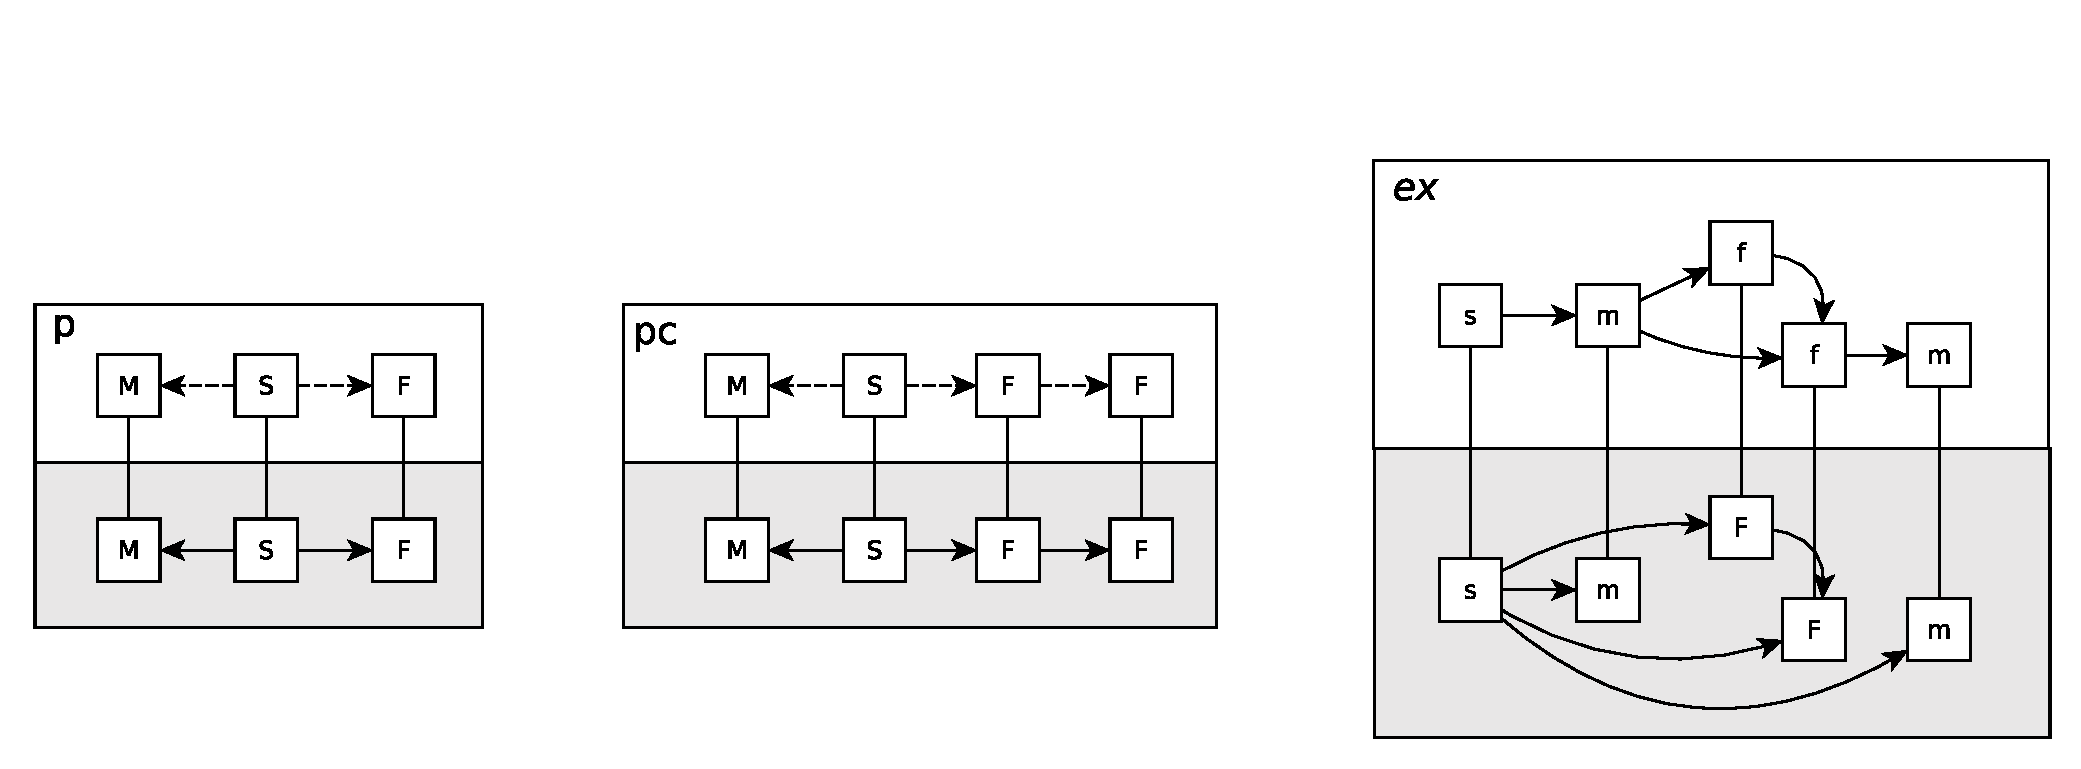
\includegraphics[scale=.35]{./figures/property_proving/proof_example.pdf}
	\caption{A Property, a Path Condition and a Transformation Execution for the Police Station Transformation}
	\label{fig:proof_example}
\end{figure}

This proof will be performed in two parts: in part 1) we will start by showing that the
premises of our proposition, $ex\Vvdash pc$ and $pc\vdash p$, imply that there
exists a typed graph injective homomorphism between $Match_p$ and
$Match^{*}_{x}$\;; in part 2) we then need to show that the premises of our proposition
and the fact that there exists a typed graph injective homomorphism between
$Match_p$ and $Match^{*}_{x}$ imply that there exists an typed graph injective
homomorphism between $p$ and $ex^*$.

Regarding part 1), let us show that $ex\Vvdash pc$ and $pc\vdash p$ imply
that there exists a typed graph injective homomorphism between $Match_p$ and
$Match^{*}_{x}$. Given that $pc\vdash p$, by 
definition~\ref{def:sat_prop_pc} we only have to consider the case where there
exists a typed graph injective homomorphism $f$ between $Match_p$ and
$Match^{*}_{pc}$. 
Given $ex\Vvdash pc$, by definition~\ref{def:instance_pc_ex} we only have to
consider the case where a typed graph injective homomorphism $g$ exists between  
$Match_{pc}$ and $Match^*_x$.
Given the above, we can conclude that there exists a typed graph injective
homomorphism between $Match_p$ and $Match^{*}_{x}$ that can be built as the
composition of $g$ and $f$, i.e. $g\circ f$. This part of the proof is
exemplified in figure~\ref{fig:proof_example_morphism_p_to_ex_match}. Note
that in the figure we have represented the transitive closure of $pc$ and $ex$ by including a different
type of dashed arrows between elements that are transitively linked.%\levi{careful about indirect links in $p$ and $pc$} 

\begin{figure}[h!] \centering 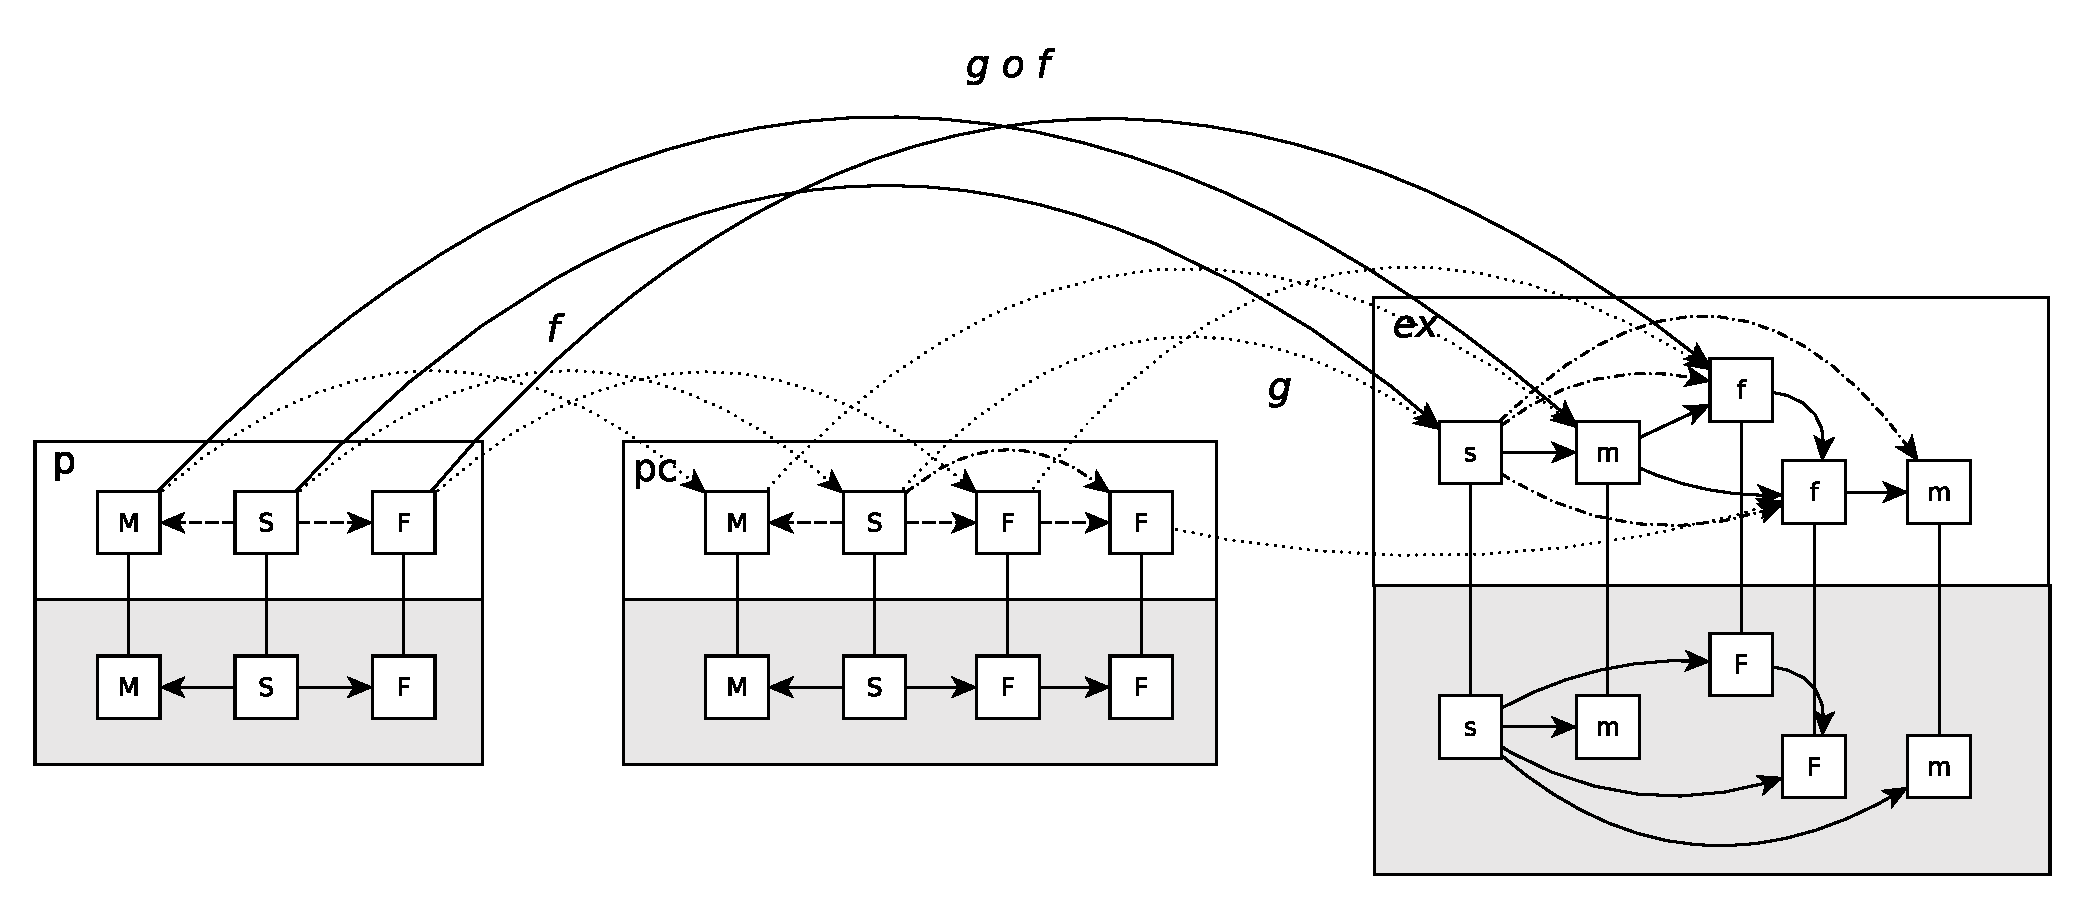
\includegraphics[scale=.35]{./figures/property_proving/proof_example_morphism_p_to_ex.pdf}
	\caption{Building the Injective Homomorphism between the Match part of a Property and a Transformation Execution}
	\label{fig:proof_example_morphism_p_to_ex_match}
\end{figure}

Regarding part 2), let us now show that the existence of a typed graph injective
homomorphism between $Match_p$ and $Match^{*}_{x}$ implies that there exists a
typed graph injective homomorphism between $p$ and $ex^*$. We have that
$pc\vdash p$ and as such by definition~\ref{def:sat_prop_pc} there exists a
typed graph injective homomorphism $k$ between $p$ and $pc^*$. We also have that
$ex\Vvdash pc$, which means that $\langle V_x,E_x\setminus E_{mx},\tau_x\rangle$
is a typed graph strict instance of $\langle V_{pc},E_{pc}\setminus
E_{mpc},\tau_{pc}\rangle$, where $Match_x = \langle V_{mx},E_{mx},\tau_{mx}\rangle$ and $Match_{pc}
= \langle V_{mpc},E_{mpc},\tau_{mpc}\rangle$.

By definition~\ref{def:typed_graph_strict_instance} this means there exists a
surjective graph homomorphism $h$ between $\langle V_x,E_x\setminus
E_{mx},\tau_x\rangle$ and $\langle V_{pc},E_{pc}\setminus
E_{pc},\tau_{pc}\rangle$. Relation $h^{-1}$, the inverse of $h$, necessarily
contains an injective typed graph homomorphism $i\subseteq h^{-1}$, given that $h$ is
type respecting. The relations involved in this part of the proof are
exemplified in figure~\ref{fig:proof_example_morphism_pc_to_ex_apply}. Note
that, since $i$ overlaps with part of $h^{-1}$, in order to make it distinct in
figure~\ref{fig:proof_example_morphism_pc_to_ex_apply}, $i$ is represented using
a thicker dashed line than the other homomorphisms in the picture. 
 
\begin{figure}[h!] \centering 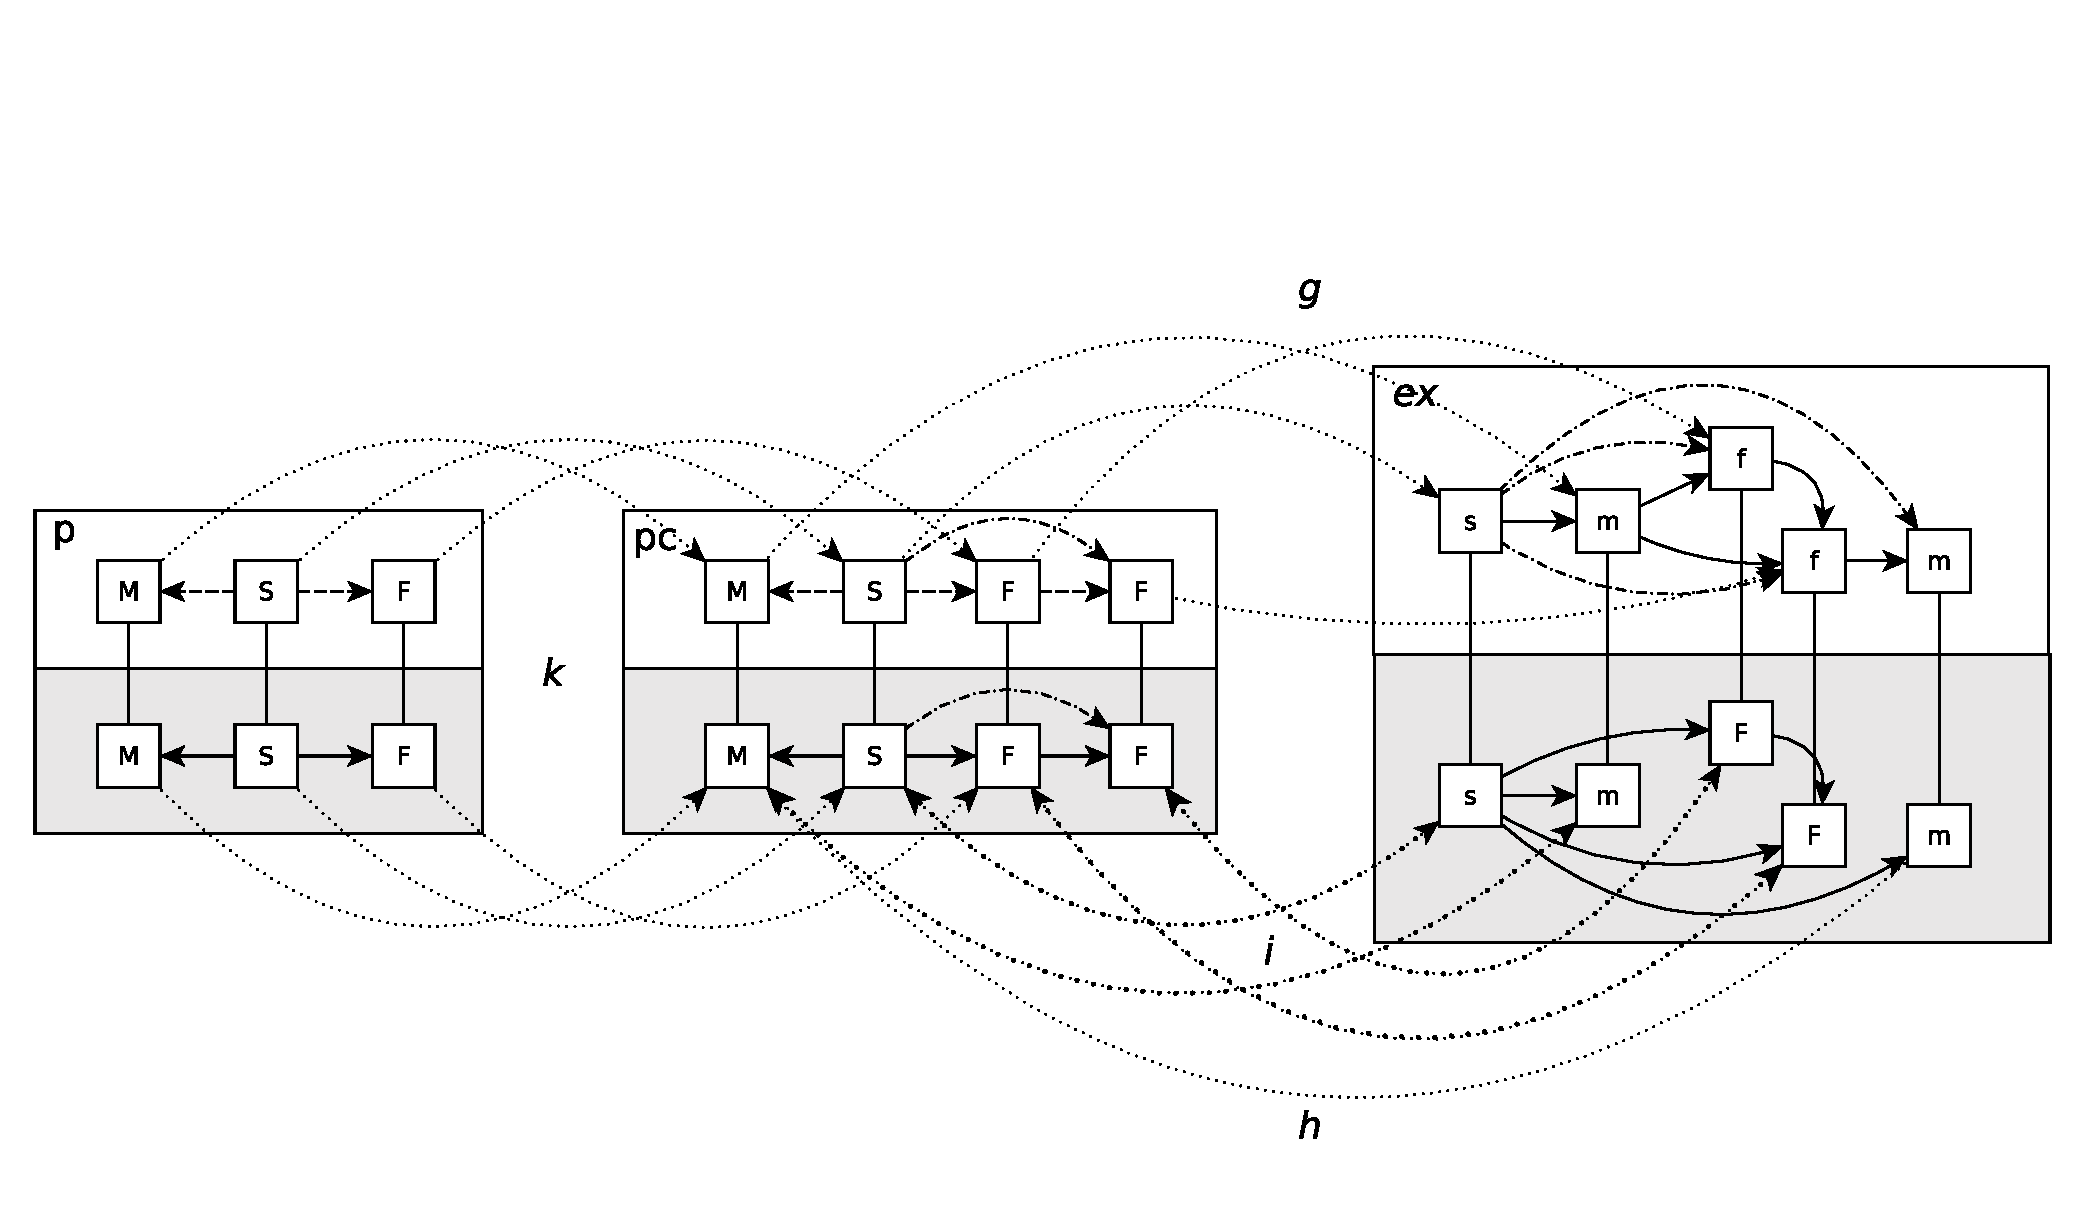
\includegraphics[scale=.35]{./figures/property_proving/proof_example_morphism_inverse_surjection.pdf}
	\caption{Building the Injective Homomorphism between the Apply part of a Path Condition and a Transformation Execution}
	\label{fig:proof_example_morphism_pc_to_ex_apply}
\end{figure}
We can thus finally build an injective homomorphism $j = g\cup i$ between $pc^*$ and
$ex^*$. This morphism is exemplified in figure~\ref{fig:proof_example_morphism_pc_to_ex}.

\begin{figure}[h!] \centering 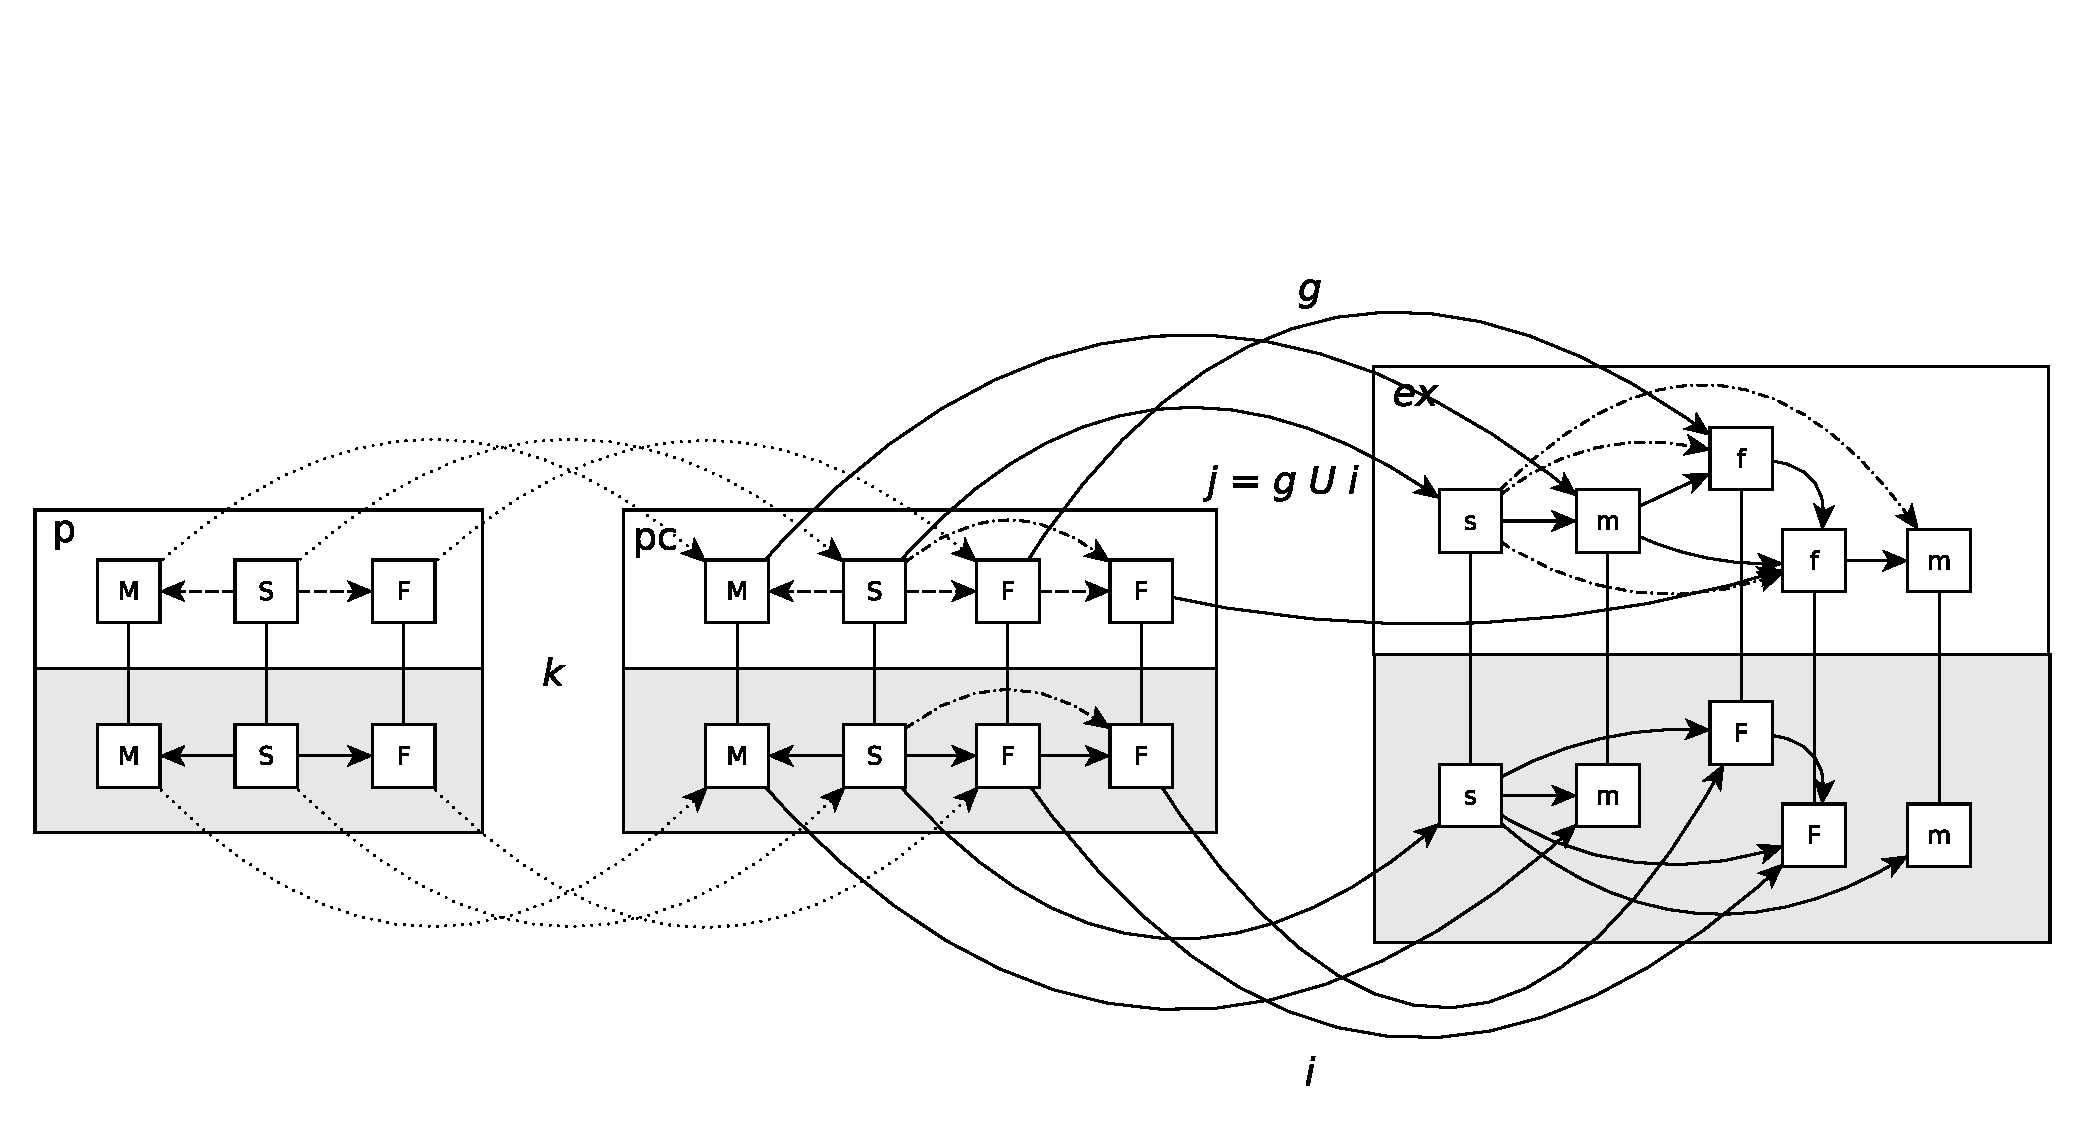
\includegraphics[scale=.35]{./figures/property_proving/proof_example_morphism_pc_to_ex.pdf}
	\caption{Building the Injective Homomorphism between a Path Condition and a Transformation Execution}
	\label{fig:proof_example_morphism_pc_to_ex}
\end{figure}

From the above we can conclude that there exists a typed graph injective
homomorphism between $p$ and $ex^*$ that can be built as $j\circ k$, the
composition of injective typed graph isomorphisms $k$ and $j$. This homomorphism is exemplified in figure~\ref{fig:proof_example_morphism_composition}.

\begin{figure}[h!] \centering 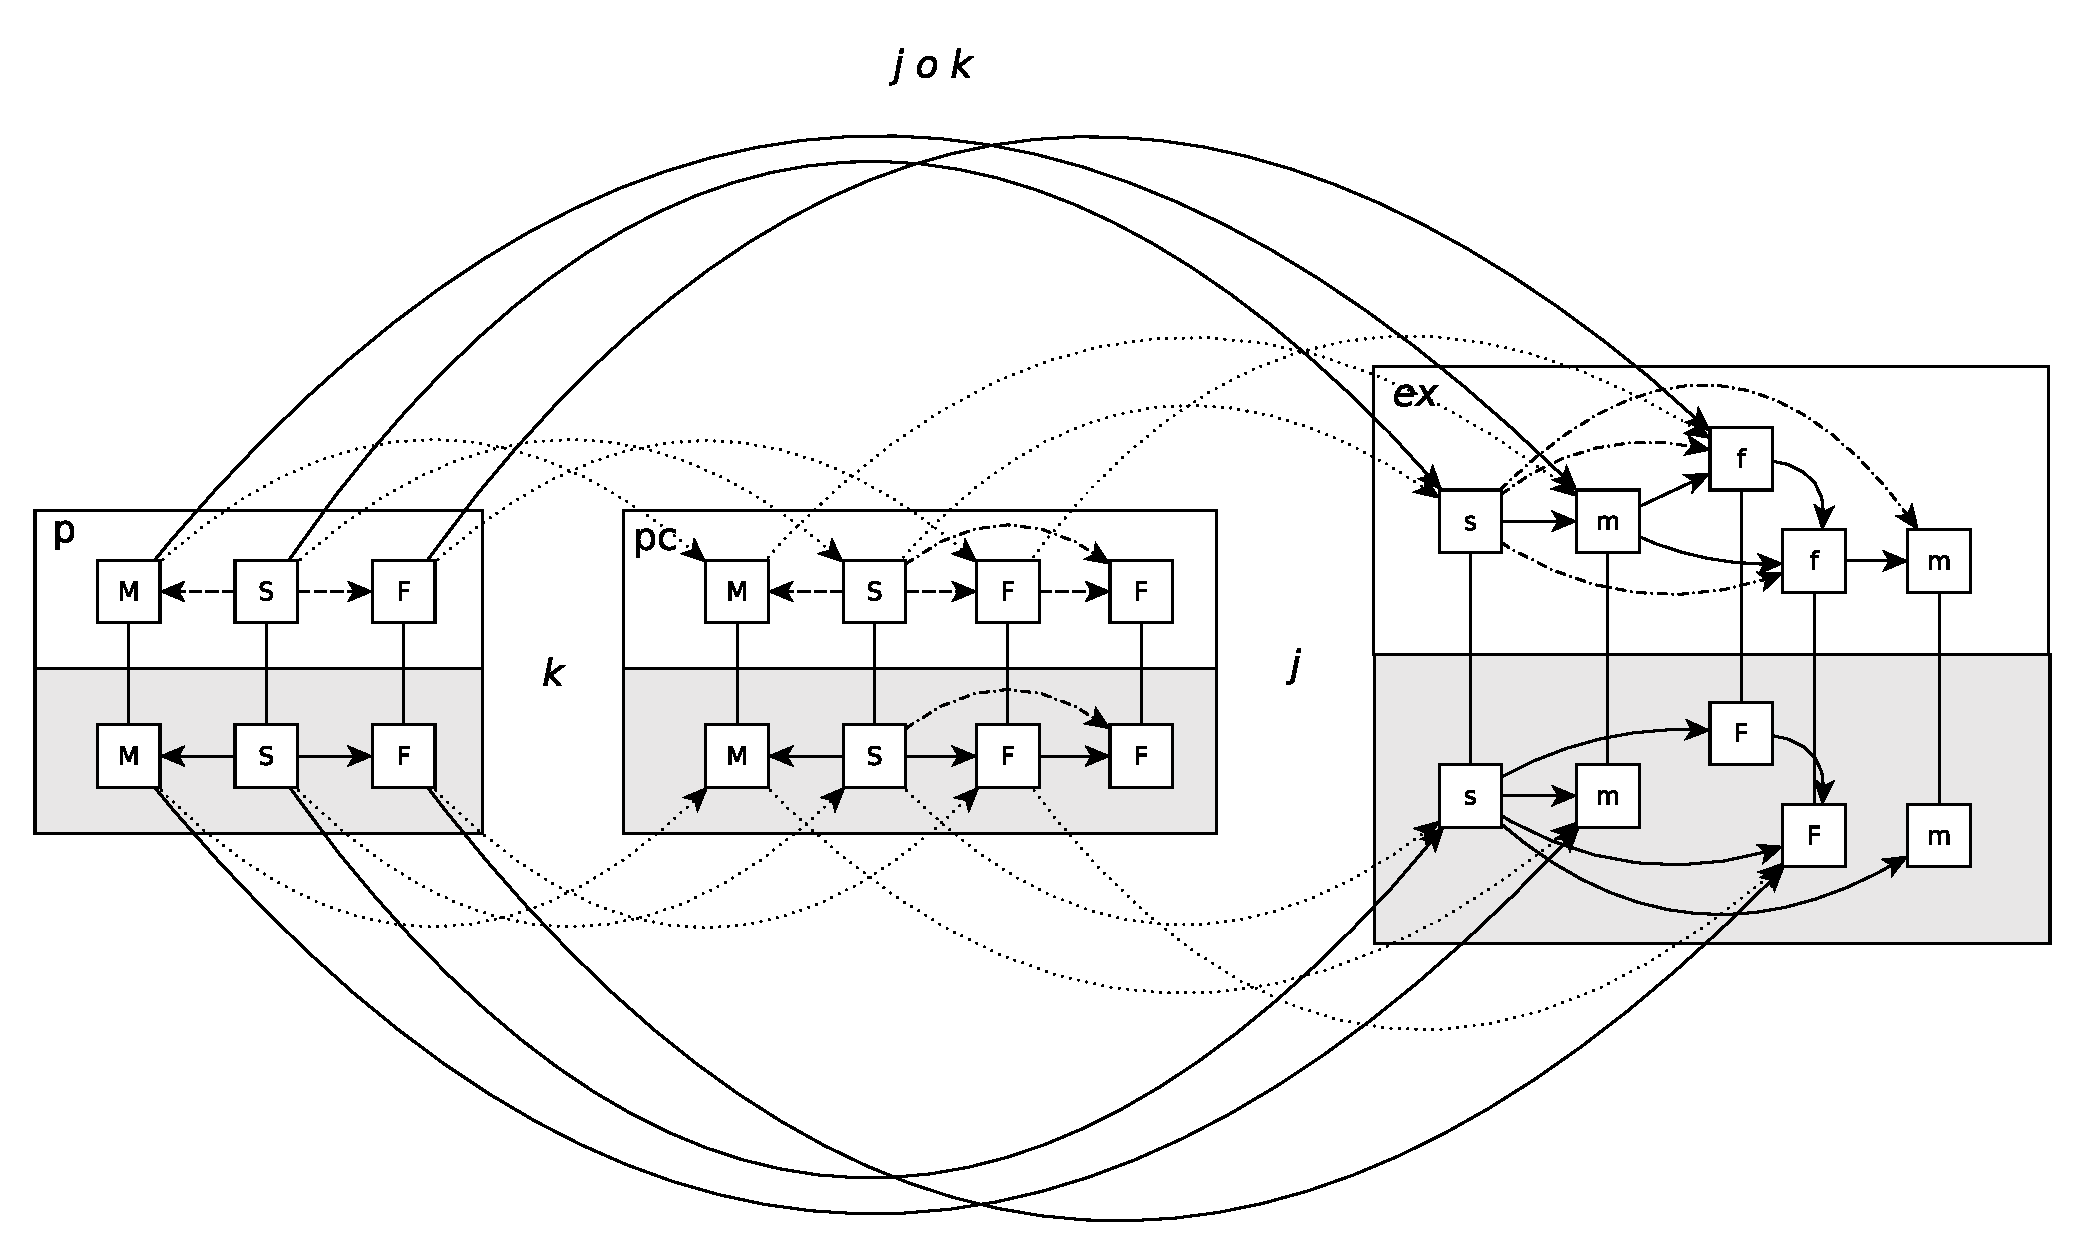
\includegraphics[scale=.35]{./figures/property_proving/proof_example_morphism_composition.pdf}
	\caption{Building the Injective Homomorphism between a Property and a Transformation Execution}
	\label{fig:proof_example_morphism_composition}
\end{figure}
\end{pf}

\begin{lemma}{If a property holds for a transformation execution then the property holds for the path condition that abstracts it.}
\label{lemma:validity2}
\end{lemma}
\begin{pf}
We will now prove the reverse direction of the implication, i.e. that:
$$ex\models p \;\Longrightarrow\;ex\Vvdash pc\land\; pc\vdash p$$
By using contraposition we can show that:
$$\neg(ex\Vvdash pc\land pc\vdash p) \;\Longrightarrow\; \neg(ex\models p)$$

We only need to worry about the case where we have  $ex\Vvdash pc\land
\neg(pc\vdash p)$ given our property proof results are meaningful only for
transformation executions which are abstracted by the path condition being
examined. In this case we have that, because $ex\Vvdash pc$, by
definition~\ref{def:instance_pc_ex} we know that there is a surjective typed
graph homomorphism between between the apply pattern of transformation execution
$ex$ and the apply pattern of the path condition $pc$. Given we know that
$\neg(pc\vdash p)$, then we know that an injective type graph homomorphism does
not exist between $p$ and $pc$. This means that, by the
definition~\ref{def:typed_graph_homomorphism} of injective typed graph
homomorphism, there exists a type $T$ which is instantiated in $pc$ but not in
$prop$. However, because of the fact that $ex\Vvdash pc$ we know that $T$ is
instantiated in $ex$ because a surjective typed graph homomorphism exists
between $ex$ and $pc$, implying type $T$ is instantiated at least once in $ex$.
We thus can deduce that we have $\neg(ex\models p)$ given that $ex\models p$
implies that there exists an injective type graph homomorphism between property
$p$ and execution $ex$. This injective type graph homomorphism cannot exist given the fact an instance
of $T$ exists in $ex$ but not in $p$.
\end{pf}

\subsubsection{Completeness}


\begin{proposition}{(Completeness) Proving that a property holds or does not
hold by examining all path conditions of the transformation is equivalent to
proving the property holds or does not hold for all transformation executions.}
\label{prop:PP_completeness}
\end{proposition}
\begin{ps}
This result follows from the combination of the validity and completeness of the
path condition algorithm, as seen in propositions~\ref{prop:pc_validity}
and~\ref{prop:completeness}, as well as the validity of the property proving
step on each path condition, as seen in proposition~\ref{prop:validity}.
\end{ps}



% \section{T-Core}
% \label{sec:t-core}
% In order to build our tool we have chosen the T-Core framework introduced by Syriani and Vangheluwe in~\cite{DBLP:journals/eceasst/SyrianiV10}. T-Core is a set of primitive model transformation blocks that can be used to replicate the behavior of existing transformation languages (e.g. in order to compare their expressiveness and provide a framework for interoperability), or to build new model transformation languages.
% 
% The framework includes five main primitive transformation blocks that exchange models and transformation information in messages called \emph{packets}. Those blocks are:
% 
% \begin{itemize}
% \item the \emph{Matcher}, that finds matches of a given pre-condition pattern within a model by running an efficient combination of the Ullmann's and VF2's subgraph isomorphism algorithm and collects those matches in a \emph{packet}
% 
% \item the \emph{Iterator} which allows selecting the next matched submodel from the set of matches gathered in a \emph{packet}
% 
% \item the \emph{Rewriter} consumes a matched subgraph from a model in a packet and changes the model according to a given post-condition pattern
% 
% \item the \emph{Rollbacker} which allows checkpointing and restoring \emph{packets} such that backtracking can be achieved
% 
% \item the \emph{Resolver} for solving potential conflicts
% between matches and rewritings
% \end{itemize}
% 
% 
% An additional T-Core construct is called the \emph{composer}, and is used to encapsulate compositions of the five primitive transformation blocks described above. The goal of the encapsulation mechanism is that complex transformation blocks, such as \emph{querying},\emph{rewriting one random match} or \emph{rewriting all matches found}, can be seamlessly created from the simplest transformation blocks.
% 
% Note that the transformation primitives described above execute transformations on models which are metamodel instances. Matching precondition patterns and rewriting postcondition patterns can only occur if the pre- and post-condition patterns are generated from the same metamodel as the models being treated. This is in order to insure coherence.